The evaluation of a drone programming system is crucial to assess its effectiveness, performance, and suitability for specific applications. 
This chapter aims to provide a comprehensive evaluation of EasyFly. 
The baseline used to compare our programming environment is the basic Crazyflie python library (cflib) 

We divided the evaluation process into two main topics: we will give a qualitative analysis of EasyFly and an understanding of the strengths and leaks of our programming system.
For this analysis, we participated in the challenges organized for the Digital Futures Drone Arena project~\cite{dronearena}.
During this challenge, groups of students and enthusiasts were asked to complete an obstacle run using Crazyflie 2.1 nano drones.

Then, we will move to performance analysis of EasyFly in a real example implementation, comparing it with a similar implementation written using only the core cflib.
This evaluation aims to assess the ease of implementing a drone application with EasyFly and the consequent reduction in complexity in the scripts. 
On the other hand, we will demonstrate that the performance of an application developed with EasyFly is almost the same as the implementation using the core cflib offered by Crazyflie.

Given the high complexity of performance evaluation of drone applications, we designed and implemented a simulation environment for EasyFly.
This simulation environment allowed us to conduct a precise performance analysis without deviating from the real environment's performance.

\section{Qualitative Analysis}\label{sec:qualitative_analysis}
In the HDI domain, the research's core part, especially from the computer science perspective,
is the experimental phase. During this phase, researchers put their ideas and prototypes to test
and assess the practicality of innovative interaction models.

For a programming environment like EasyFly, testing and evaluating in a real research scenario in HDI is essential. 
The testing in real scenarios can help detect possible weaknesses in the programming environment, allowing for fine-tuning the model.

To best evaluate our EasyFly programming environment, we had the possibility to participate in the Digital Futures Drone Arena project~\cite{dronearena}.

The Drone Arena project planned two challenges where groups of students and enthusiasts with different backgrounds were asked to complete a specific task using drones.
These challenges aim to allow researchers to collect data and perform studies about human-drone interactions.

The EasyFly programming environment was part of the inaugural challenge in Sweden in June 2022~\cite{dronearenaChallenge}. 
In this challenge, five groups of students and enthusiasts with knowledge of computer science were asked to program Crazyflie 2.1 nano drones to complete an obstacle course.
There were two main alternatives to write the scripts: the standard cflib or the EasyFly programming environment. 

The challenge was distributed over three days; the first two days were dedicated to development and testing, and the last day was dedicated to the final challenge, where the groups competed with each other with what they had produced in the days before.
On the first day, we gave the groups a brief presentation on the basic knowledge of the Crazyflie 2.1 platform. 
We also described the main components and working principles of the EasyFly programming environment.
Then, we provided the groups with a Python project, where inside was the original cflib, our EasyFly programming environment, and a folder of examples for both.
From then on, the groups were free to develop and test the code with real Crazyflie 2.1 in a sample stage, with minimum support from the research team.

This particular setting of the challenge allowed us to see and measure the impact of using EasyFly on a group with minimum knowledge of the Crazyflie platform. 
On the final day of the challenge, 2 out of 5 teams decided to participate in the final using our EasyFly programming environment. 

The approach for all the groups was to use a Multiranger deck and perform a hand-driven flight through the obstacle course.
The main differences were how the groups implemented the mechanism that allowed them to push or pull the drone using their hands.

By analyzing the code that all the groups produced, we noticed two main aspects of the usage of the EasyFly programming environment:
The groups that started using EasyFly from the beginning developed more complex solutions.
The code of the groups that used the programming environment looked clean and simple, even if the solution they implemented was more complex.

Although we expected more adhesion on EasyFly, we noticed that almost all the groups had a look at the code of the programming environment, in particular inside the utility functions of the ECF modules. 
In their final code, almost every group used the utility functions of the Multiranger ECF Module, either directly or indirectly.

In conclusion, the challenge of the Drone Arena project allowed us to understand that the entire EasyFly programming environment, particularly the Coordination Manager, can seem too complicated at first glance and was a little more complex than we thought.
The groups that decided not to use the programming environment decided on purpose to develop a more simple and sometimes effective solution.


\section{Performance Analysis}\label{sec:performance_analysis}

EasyFly is a programming environment that aims to ease the development of drone applications, reaching the same solution with less effort, both in terms of time to write the solution and expertise required to implement the solution.
Even if simplicity remains the first objective, performance plays an important role in the EasyFly programming environment.
If the programming environment is easy to use but, in the end, results in inefficiency in terms of performance, it automatically becomes useless.

To assess the performance of EasyFly, we compared it with the standard implementation of Crazyflie's cflib across two real example applications used in HDI research.
The first application scenario takes place in an artistic exhibition between a human performer and a drone. 
The second application scenario is an obstacle course similar to the Drone Arena inaugural challenge~\cite{dronearenaChallenge}.

In this analysis, we will demonstrate that the expected loss in performance with respect to the basic cflib implementation is shallow compared to the reduction of program complexity.

\subsection{EasyFly Simulation Environment}\label{subsec:simulation_environment}
Measuring performance in drone applications is a very hard task, and usually, the performance of the applications can vary highly across different runs.
When running the application in a real environment, the performance of the applications can usually vary highly across different runs.
Given the fact that the conditions of the environment influence performance, the only possible strategy to measure performance is to execute and sample the same scenario multiple times and then average the results.
Of course, this approach can have a high cost in terms of time and resources consumed.

To simplify the evaluation process and collect more precise data, we developed a simulation environment for EasyFly.
In the simulation environment, the drones are replaced by a virtual copy that replicates the drone's movements in a controlled simulation.
The simulation allows the reduction of the influence of the environment on performance measurements to zero, enabling precise performance measurement with a single run.
This approach drastically reduces the costs of the analysis.
A possible drawback of a poorly accurate simulation environment is that the performance can deviate from the real application performance.

In our simulation environment, we create a virtual Crazyflie 2.1 that emulates a real Crazyflie 2.1.
Upon receiving the commands from the ground station, the virtual Crazyflie computes and updates its internal state (position, velocity, acceleration, and some sensor measures) and sends back data.
In the current implementation of the EasyFly simulation environment, the virtual Craziflie emulates the control-related commands, logging, and parameter features.

As shown in Figure~\ref{fig:simulation_environment}, the virtual Crazyflie communicates with the ground station's script using a UDP channel.
Usually, the ground station script and the simulated Crazyflie run on the same machine, so the UDP communication is local.

The script of the ground station is entirely independent of Crazyflie's software. 
The execution and performance of the ground station's script are not affected by whether the Craziflie is virtual or not.
This separation guarantees that the performance measured with EasyFly's simulation environment does not deviate from the real environment.

\sidecaptionvpos{figure}{b}
\begin{SCfigure}[\sidecaptionrelwidth][h]
    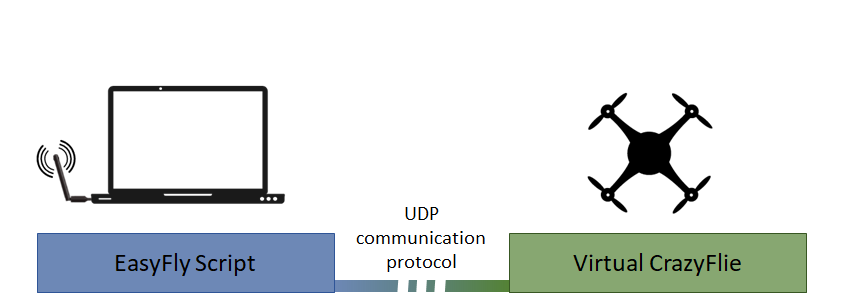
\includegraphics[width=0.5\textwidth]{evaluation/simulation_environment}
    \caption{Structure of EasyFly simulation environment}\label{fig:simulation_environment}
\end{SCfigure}


\subsection{Application Scenario Evaluated}\label{subsec:application_scenario_evaluated}
To best evaluate the performance of any system, it is crucial to select the appropriate application scenario.
In particular, it is essential to test the system in a scenario that is as close as possible to an actual application of this system.

Given that our programming environment is designed to build drone applications for HDI research, we selected two representative application scenarios from the literature on HDI.

The first application takes inspiration from recent research conducted in the field of HDI~\cite{eriksson2020ethicsInMovement}. 
This research explored how ethicality is shaped in the interaction between a choreographer, a performer, and a choir of five drones performing together on the opera stage.
In our simplified version of this scenario, we reduced the drones to a single drone. 
Moreover, the choreography designed for the drone is determined before the performance.
In other words, our drone should follow a predetermined path on the stage, exhibiting with the performer. 
The drone should also implement an obstacle avoidance mechanism to avoid any collision on the stage.
In Figure~\ref{fig:exhibition}, we can see the trajectory followed by the virtual Crazyflie during the performance measurement of this application.

The second application we selected for performance analysis is an obstacle course similar to the one adopted for the inaugural challenge of the Digital Futures Drone Arena project~\cite{dronearenaChallenge}.
In this application, we based the implementation of the algorithm on an elevation model of the environment. 
In other words, we modeled the obstacle course stage with a grid where every cell contains the elevation at that coordinate.
We then implemented a script to navigate safely in the provided environment. 
We also adopted the obstacle avoidance mechanism in this application to avoid unpredicted crashes.
In Figure~\ref{fig:obstacle_course}, we can see the trajectory followed by the virtual Crazyflie during the performance measurement of this application.

\begin{figure}[t]
    \centering
    \subfloat[Frist application scenario: drone exhibition\label{fig:exhibition}]{
        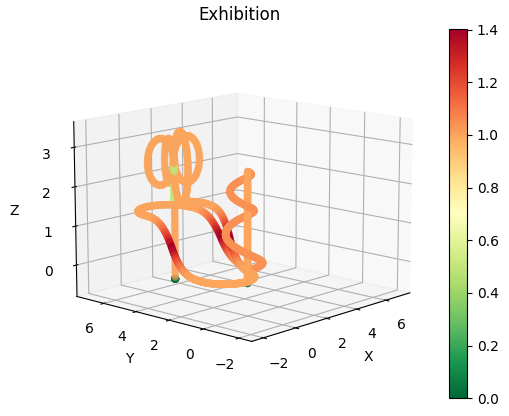
\includegraphics[width=0.45\textwidth]{evaluation/exhibition}
    }
    \quad
    \subfloat[Second application scenario: drone obstacle course\label{fig:obstacle_course}]{
        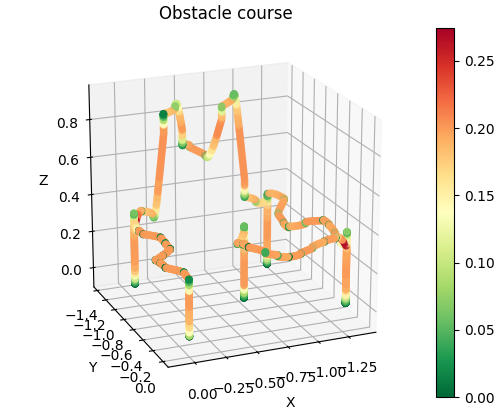
\includegraphics[width=0.45\textwidth]{evaluation/obstacle_course}
    }
    \caption{Application scenarios' trajectories}\label{fig:application_traj}
\end{figure}

\subsection{Tools and Metrics for Measuring Performances}\label{subsec:performance_metrics}
As previously anticipated, our core objective is to produce a simple programming environment; given this, the most critical analysis is around the complexity of the applications.
Another important aspect to keep under control is the execution performance 

To evaluate our programming environment, we indeed targeted two main categories of performance metrics: complexity and execution performance.

The first category, complexity, is composed of a set of metrics that tries to evaluate the complexity of a program.
The category is composed of the following metrics:
\begin{itemize}
    \item Lines of Codes (LOC)
    \item Cyclomatic Complexity (CC)
    \item Halstead Metrics (HAL)
\end{itemize}

The LOC metric is the most simple measure of the complexity of a program. As the name suggests, it is the count of lines of code of the program under analysis.

The Cyclomatic Complexity is a Complexity analysis method proposed by Mccabe in 1996; it evaluates the complexity by measuring the number of linearly independent paths
through a piece of code~\cite{mccabe1996cyclomatic}.

The Halstead Metrics was introduced by Maurice H. Halstead in the 1970s. 
They are based on the analysis of the number of unique operators and operands in a program, as well as their occurrences~\cite{hariprasad2017software}.
The five main metrics proposed by Halstead are:
\begin{itemize}
    \item \textbf{Program Vocabulary} (\( \eta \)): The total number of unique operators and unique operands in the program. 
    It is given by the formula: \( \eta = \eta_1 + \eta_2 \) where \( \eta_1 \) is the number of distinct operators, and  \( \eta_2 \) is the number of distinct operands.
    \item \textbf{Program Length} (\( N \)): The total number of operator occurrences and operand occurrences in the program. It is given by the formula: \( N = N_1 + N_2 \), where \( N_1 \) is the total number of operators and \( N_2 \) is the total number of operands.
    \item \textbf{Program Volume} (\( V \)): A measure of the size of the program. It is given by the formula: \( V = N \log_2 \eta \).
    \item \textbf{Program Difficulty} (\( D \)): Represents the complexity of the program. It is given by the formula: \( D = \frac{\eta_1}{2} \cdot \frac{N_2}{\eta_2} \).
    \item \textbf{Effort} (\( E \)): Represents the effort required to understand and develop the program. It is given by the formula: \( E = D \cdot V \).
\end{itemize}

To collect all these measurements, we used \textit{radon}~\cite{radon}, a Python library that computes all such metrics using static analysis on the source code of the scripts.

The second category of metrics, the execution performances, is a set of metrics that measures the resource consumption of the scripts.
The category is composed of the following metrics:
\begin{itemize}
    \item Memory (RAM) consumption
    \item Average CPU consumption 
    \item Max CPU consumption
    \item Network load
\end{itemize}

These metrics provide valuable insights into the efficiency and resource utilization of the scripts. 
Memory consumption indicates how much random access memory is being used. 
Average CPU consumption gives an idea of the overall CPU usage over a period, max CPU consumption highlights the peak CPU usage, and network load measures the amount of data transmitted over the network during script execution.

Analyzing these metrics is crucial for identifying potential bottlenecks and ensuring resource utilization does not constrain our programming environment.

The machine used to run the performance analysis mounts an AMD Ryzen 7 5700U with Radeon Graphics with 8GB of RAM.
To measure the memory consumption, we used \textit{memory-profiler}~\cite{memoryProfiler}, a Python library for collecting RAM usage while executing a Python script.
We used the \textit{Performance Monitor} tool for Windows for the CPU metrics. 
Finally, the simulation environment automatically computes the network load by summing all the CRTP received and sent.

\subsection{Results Analysis}\label{subsec:result_analysis}
This section will present the complexity and performance analysis results aimed at evaluating our EasyFly programming environment.

As described in Section~\ref{subsec:application_scenario_evaluated}, we selected two application scenarios that best represent our target application.
Since our primary goal is to produce a simple programming environment that researchers of HDI can use, this evaluation tries to asses the simplicity of the environment while not losing too much in performance. 

As we have seen in Section~\ref{subsec:performance_metrics}, we divided the evaluation into two categories:
\begin{itemize}
    \item Complexity analysis
    \item Performance analysis
\end{itemize}

The complexity analysis represents the core part of the evaluation and is composed of three metrics:
\begin{itemize}
    \item Lines of Codes (LOC)
    \item Cyclomatic Complexity (CC)
    \item Halstead Metrics (HAL)
\end{itemize}


Looking at the results, it is crystal clear that our programming environment, EasyFly, is much less complex than the original cflib we selected as a baseline for comparison.
Starting from the most straightforward metric, LOC, we can see in Figure~\ref{fig:loc_count} that the results are, in both scenarios, halving the count.
EasyFly, with respect to cflib, allows you to write the same application with half of the code.

By looking at the second metric, CC, we can see, also in this case, the same trend.
Moreover, when comparing the CC across the two different scenarios, it is evident that the performance gap between cflib and EasyFly increases with complexity.
In Fact, in the second scenario, the obstacle course, the total CC computed is 50\% less than the cflib's implementation.

The last metric for complexity, HAL, by looking at the results in Table~\ref{table:HAL}, confirms what we previously said for LOC and CC. 
In particular, in this case, it is much more evident that the performance gap between cflib and EasyFly increases with complexity.
Here, for the Effort (\( E \)), we observed a gap of over 55\% for the second scenario.
\begin{figure}[t]
    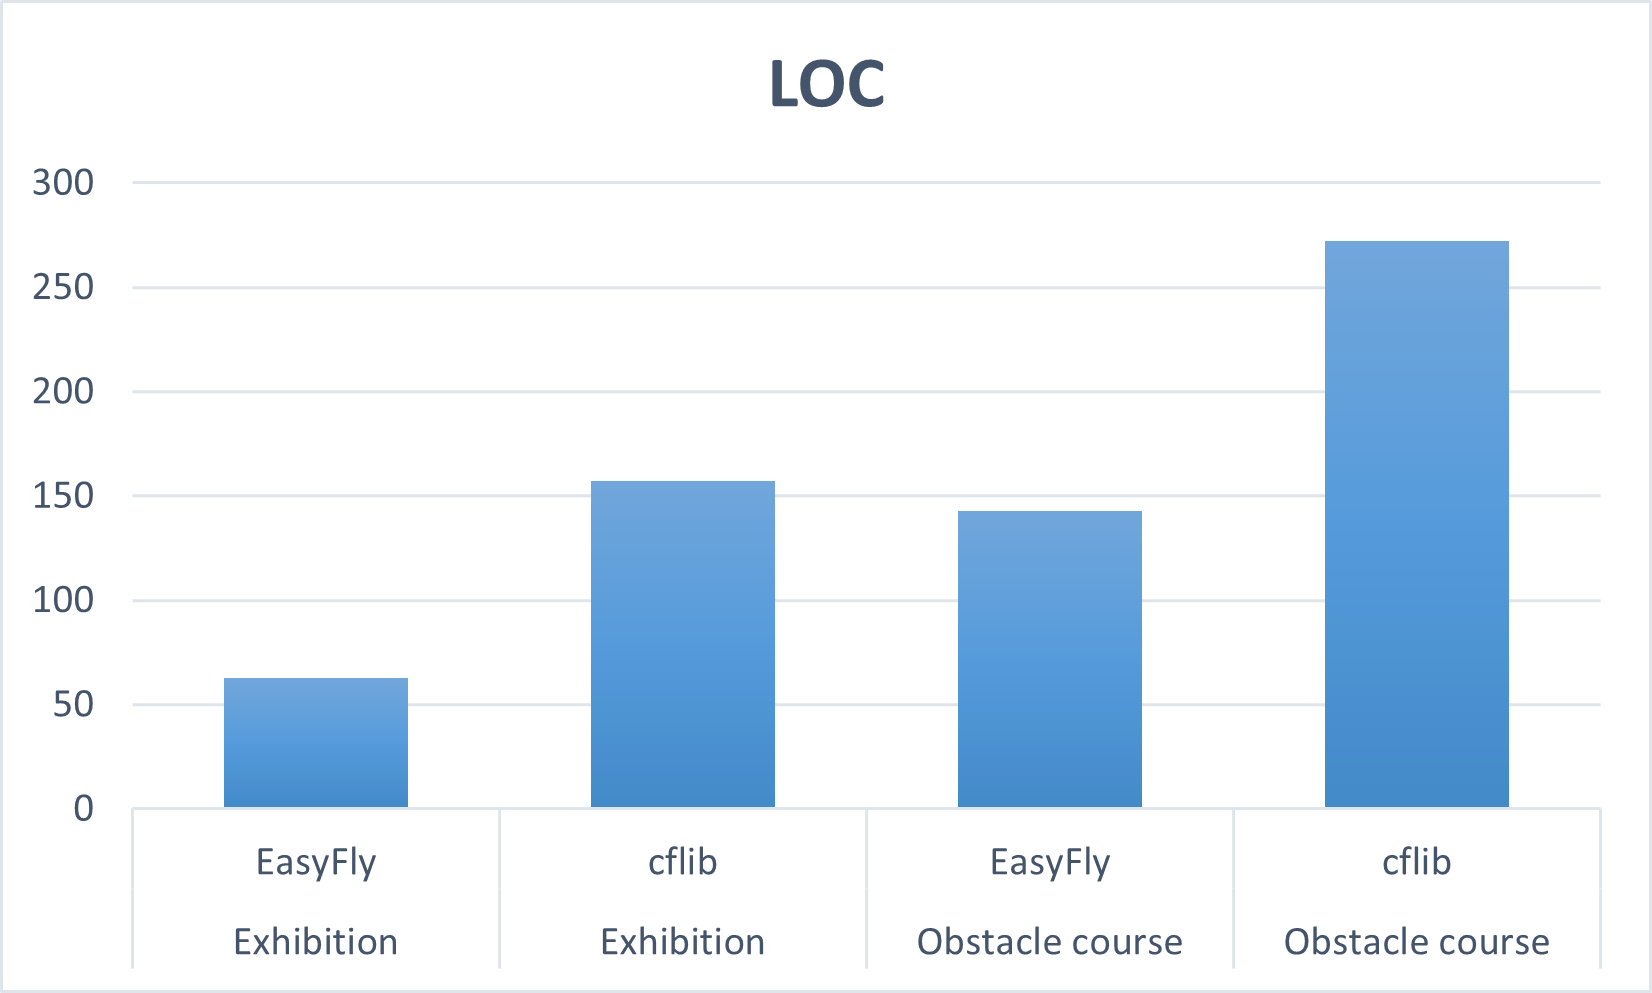
\includegraphics[width=0.6\textwidth]{evaluation/loc}
    \caption{Lines of Code}\label{fig:loc_count}
\end{figure}

\begin{figure}[t]
    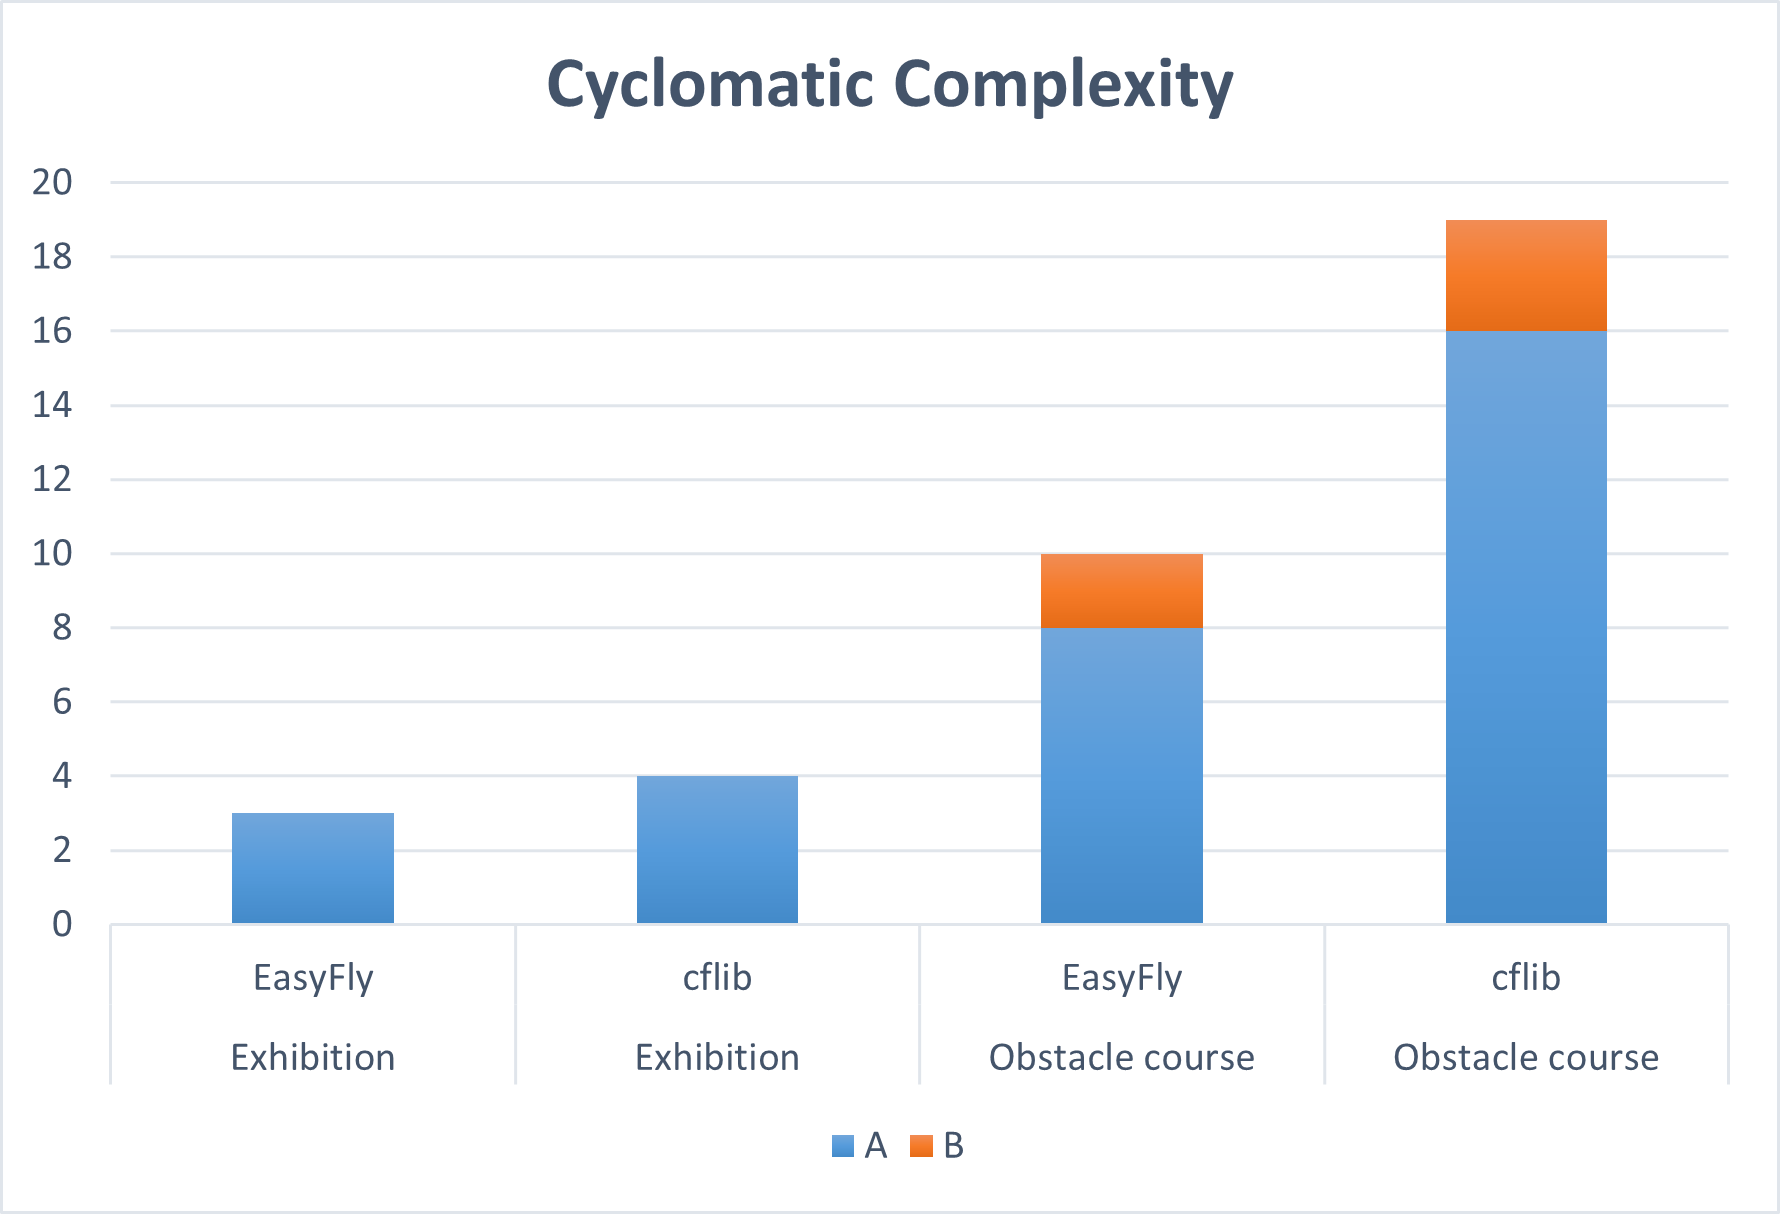
\includegraphics[width=0.6\textwidth]{evaluation/cc}
    \caption{Cyclomatic Complexity}\label{fig:cc}
\end{figure}

\begin{table}[H]
    \centering
        \begin{tabular}{*{6}{|c}|}
        \hline
        \rowcolor{bluepoli!40}
        \textbf{Scenario} & \textbf{\( \eta \)} & \textbf{\( N \)} & \textbf{\( V \)} & \textbf{\( D \)} & \textbf{\( E \)}\\
        \hline \hline
        Exhibition with cflib & 33 & 45 & 226.99 & 4.04 & 916.72 \\
        \hline
        Exhibition with EasyFly & 38 & 48 & 251 & 3.0 & 755.70 \\
        \hline \hline
        Obstacle course with cflib & 171 & 296 & 2195.68 & 8.74 & 19187.76 \\
        \hline
        Obstacle course EasyFly & 108 & 168 & 1134.82 & 7.66 & 8696.31 \\
        \hline
        \end{tabular}
        \\[10pt]
        \caption{Halstead Metrics}\label{table:HAL}
\end{table}





\begin{table}[H]
    \centering
        \begin{tabular}{*{3}{|c}|}
        \hline
        \rowcolor{bluepoli!40}
        \textbf{Scenario} & \textbf{CPU Average (\%)} & \textbf{CPU MAX (\%)} \\
        \hline \hline
        Exhibition with cflib & 0.570 & 12.829 \\
        \hline
        Exhibition with EasyFly & 0.266 & 16.449 \\
        \hline \hline
        Obstacle course with cflib & 0.540 & 18.423 \\
        \hline
        Obstacle course EasyFly & 0.625  & 22.340 \\
        \hline
        \end{tabular}
        \\[10pt]
        \caption{CPU consumption}\label{table:cpu_consumption}
\end{table}


\begin{figure}[t]
    \centering
    \subfloat[Scenario: exhibition with cflib\label{fig:mem_ex_cflib}]{
        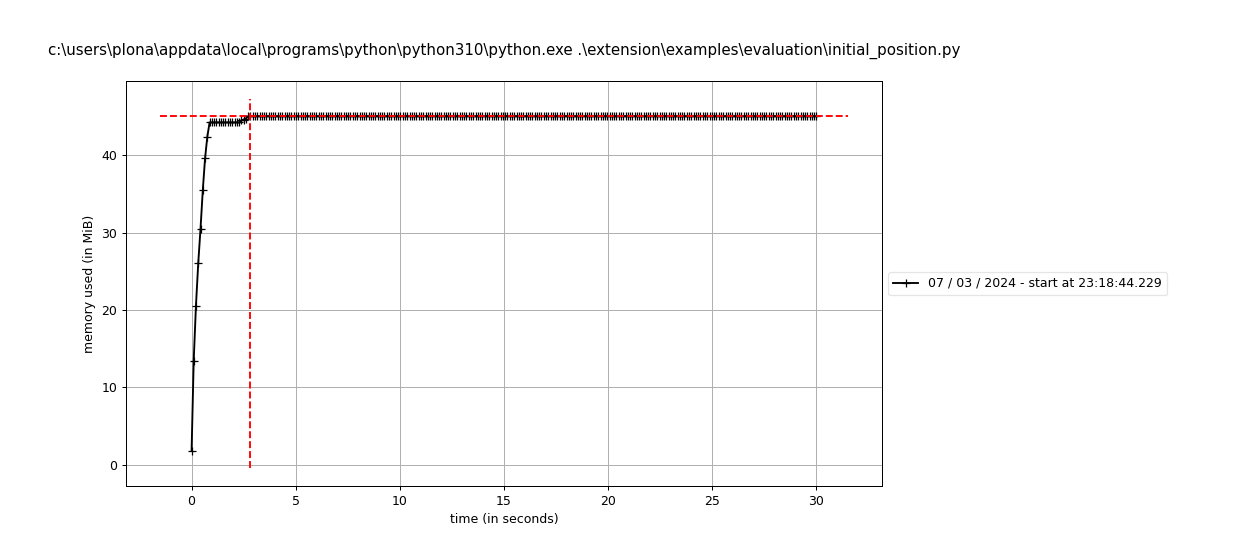
\includegraphics[width=0.45\textwidth]{evaluation/exhibition_cflib_mem}
    }
    \quad
    \subfloat[Scenario: exhibition with EasyFly\label{fig:mem_ex_ecf}]{
        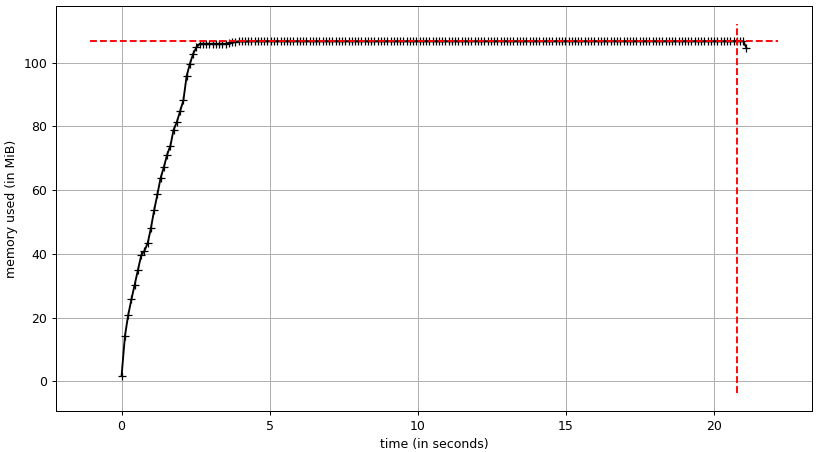
\includegraphics[width=0.45\textwidth]{evaluation/exhibition_ecf_mem}
    }
    \quad
    \subfloat[Scenario: obstacle course with cflib\label{fig:mem_obs_cflib}]{
        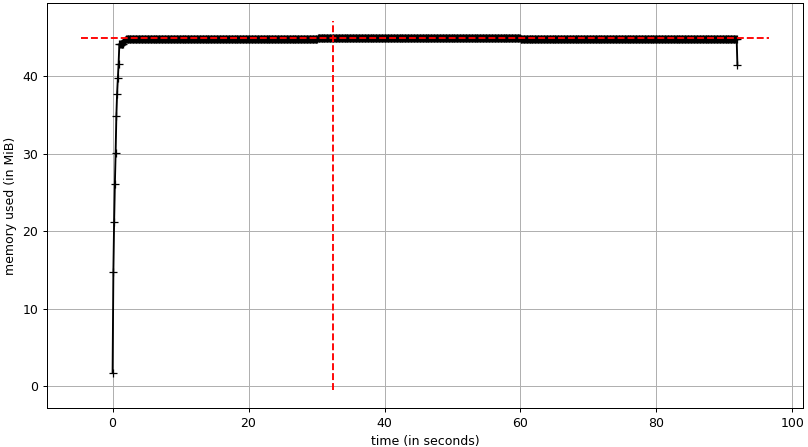
\includegraphics[width=0.45\textwidth]{evaluation/obstacle_course_cflib_mem}
    }
    \quad
    \subfloat[Scenario: obstacle course with EasyFly\label{fig:mem_obs_ecf}]{
        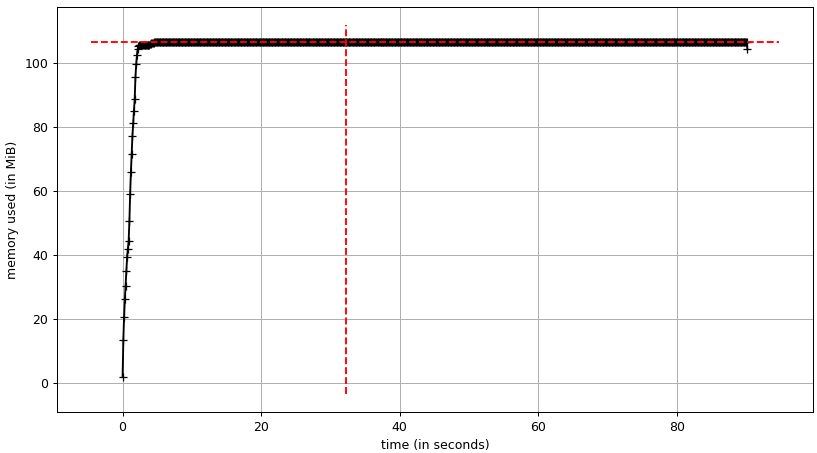
\includegraphics[width=0.45\textwidth]{evaluation/obstacle_course_ecf_mem}
    }
    \caption{Memory (RAM) usage}\label{fig:ram_usage}
\end{figure}





\begin{figure}[t]
    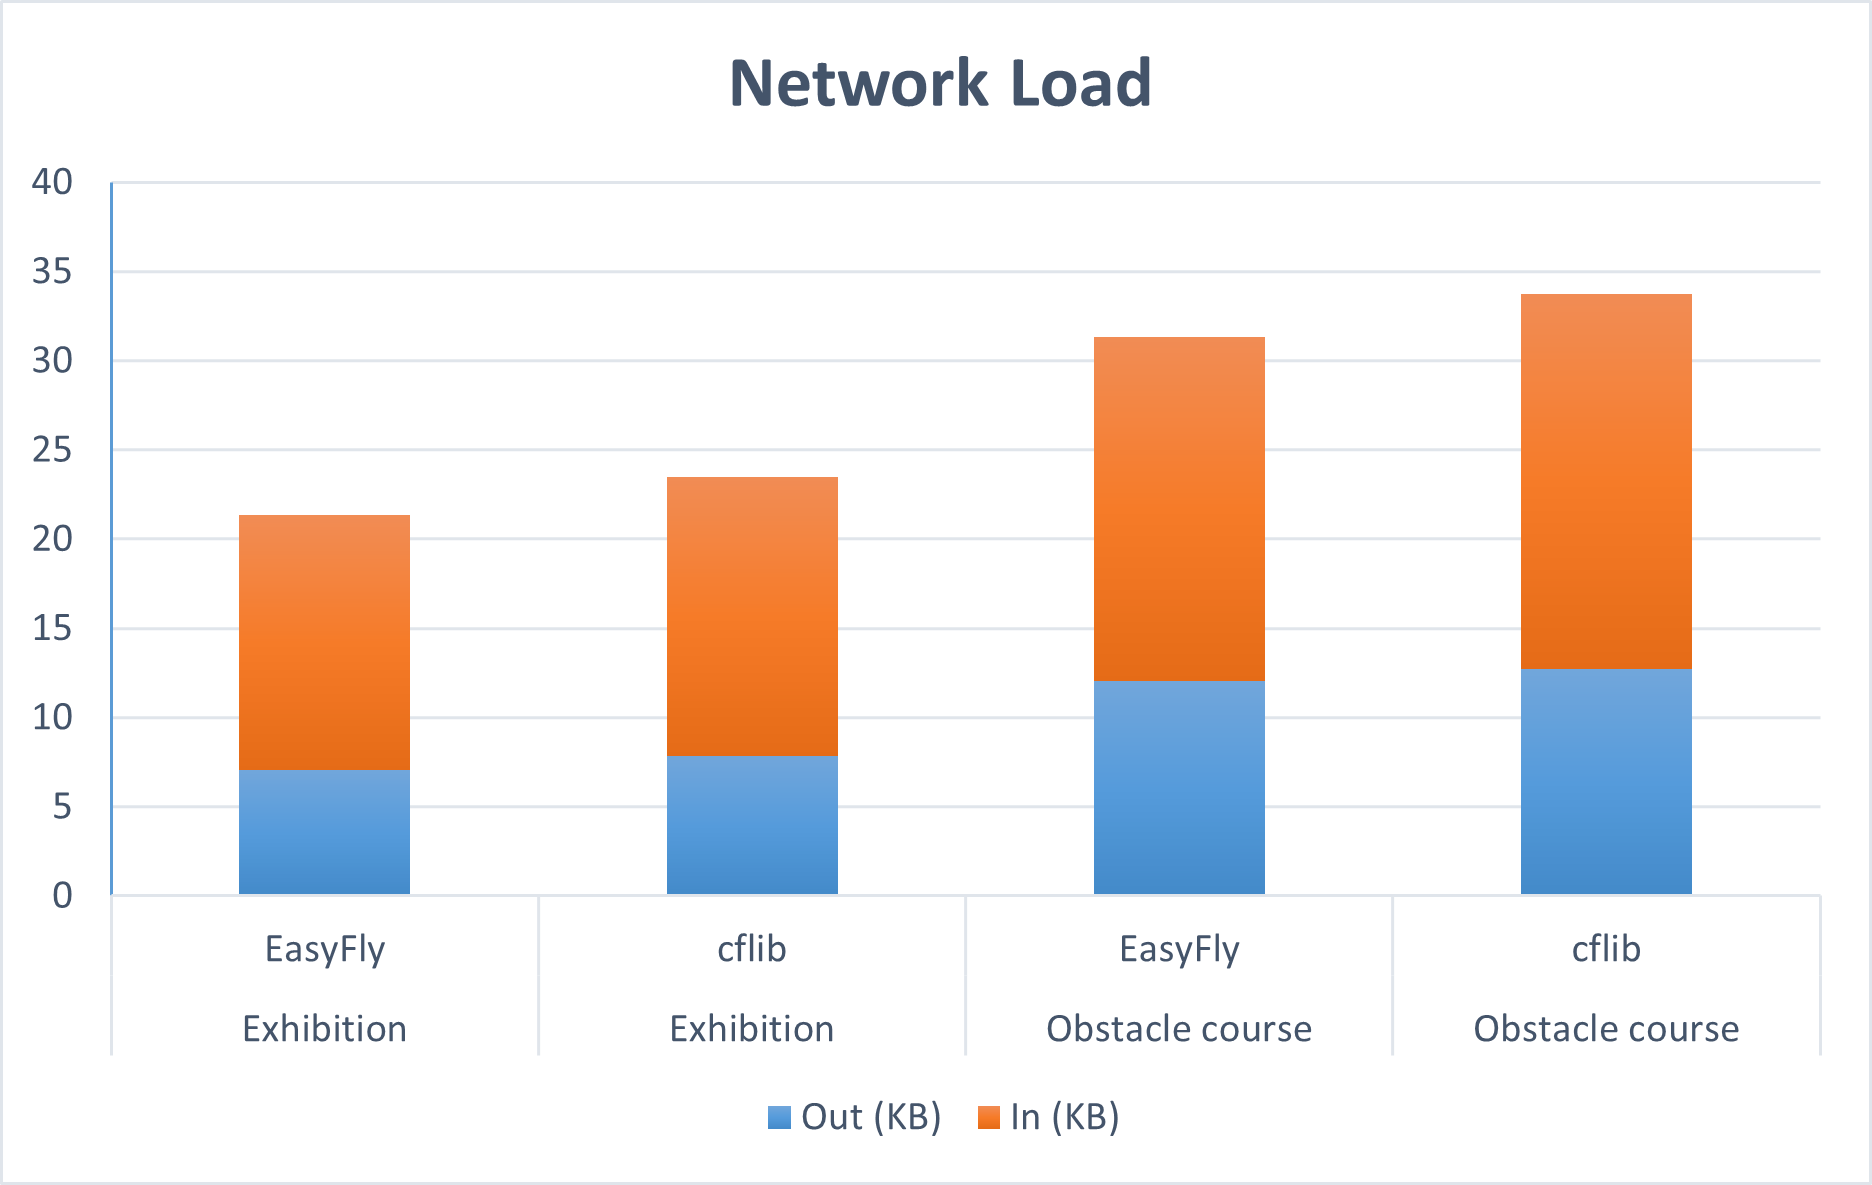
\includegraphics[width=0.6\textwidth]{evaluation/network}
    \caption{Network load}\label{fig:network_load}
\end{figure}




\subsection{Future Developement}\label{subsec:future_developement}

